\section{Introduction}
\label{sec:introduction}

Vision--language--action (\vla) models are moving robot control from fixed task
programs toward policies that translate language and multimodal observations
directly into continuous actions~\cite{pi05,rth2024}.  In the action-only
interface studied here,
each policy call returns an ordered \actionblock to a consumer, which dispatches
the block and then replans from a new observation.  This block is the first
concrete object that leaves the learned policy and becomes eligible for physical
execution; it is therefore a natural security boundary
(Figure~\ref{fig:motivation}).

\begin{figure}[!t]
\centering
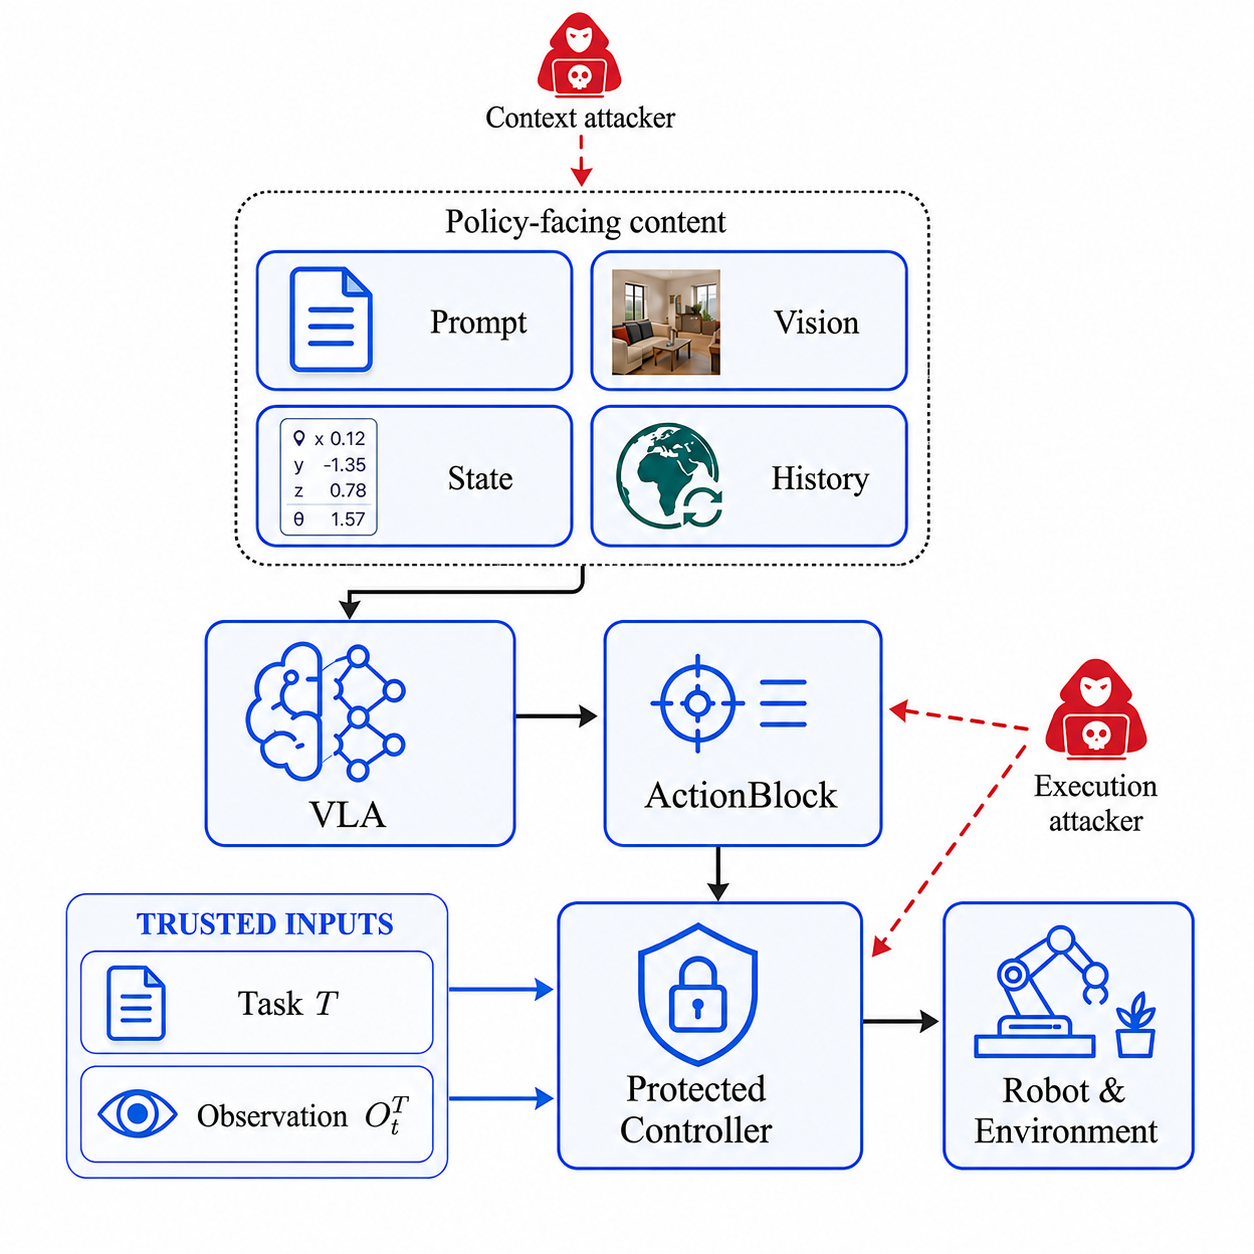
\includegraphics[width=.98\columnwidth]{figures/motivation_boundary_raster_v2_square.png}
\caption{Deployment and protection overview.  Attacks may corrupt policy inputs
or tamper with post-inference execution.  \system mediates the point at which a
newly generated continuous \actionblock becomes executable.}
\label{fig:motivation}
\end{figure}

That boundary is exposed from both sides.  Instruction perturbations, visual
perturbations, and embodied-agent jailbreaks can change the action produced by a
\vla~\cite{saber2026,freezevla2025,badrobot2025,robopair2025}.  In the motivating
SABER case, the authoritative task is to move a soda can to a plate, while the
policy is induced to act on ``move to the farthest fixture.''  The consumer sees
only the resulting numeric block, not a trustworthy account of which task
authorized it.  After inference, compromised software can additionally replace
the proposal, replay an earlier permission, reorder steps, or splice evidence
from different proposals~\cite{diat2019,cfaplus2024,arto2026,tat2026}.  An input
attack and an execution attack thus meet at the same actuator-facing object.

Existing defenses protect important parts of this path.  Structured-input and
trusted-agent architectures protect instruction/data separation or derive
digital control flow from a trusted query~\cite{struq2025,secalign2025,
camel2026,ace2026}.  Action attribution and trajectory auditing explain tool
calls or mobile-agent behavior~\cite{attriguard2026,mate2026}.  \vla verifiers
assess plan--action consistency or learned alignment over action candidates
~\cite{sealvla2026,covervla2026}.  CPS integrity and robot-attestation systems
bind protected programs, reference motion, or control flow to execution
evidence~\cite{diat2019,cfaplus2024,arto2026,tat2026}; prediction and shielding
qualify candidate consequences or continuous safety sets
~\cite{vlmpc2024,safetychance2024,measurementrobustcbf2021,
realizableshields2025}.

These defenses stop at different points around the online \actionblock.  Input
and agent defenses do not establish that the block later accepted by the robot
is the one justified by trusted task state.  Candidate verifiers may rank or
score a policy proposal, but do not preserve that verdict through ordered
dispatch and observed effects.  Execution-integrity systems begin from a
protected program or previously specified motion, while shields qualify a
physical constraint without connecting the decision back to task-relative
authority.  The surveyed defense families therefore protect different segments
of the path.  Their stated mechanisms do not jointly bind independently anchored
task authority to the exact newly generated block, its ordered dispatch, and
registered execution evidence.

This missing composition exposes two alignment gaps.  The \emph{intent--action
authorization gap} lies between trusted task intent and the exact \actionblock
generated from an attackable policy view.  The \emph{action--execution
realization gap} lies between an admitted block and its ordered dispatch,
evidence, and state-dependent physical realization.  C1 belongs to the first
stage.  C2 and C3 are the transaction-integrity and guarded-realization
obligations within the second stage.

The core question is how an action-only consumer can establish
checker-relative task authorization for an exact source block and preserve that
authorization through qualified execution without modifying the \vla.

The key insight is to treat the exact online \actionblock as the stable identity
anchor across the entire lifecycle.  Evidence attaches to this observable
object, avoiding assumptions about the model's latent intent or a unique
reference trajectory.  A scoped task-relative assessment names the source
block, the same proposal persists through dispatch and effect evidence, and any
state-dependent execution configuration is recorded separately.  Physical
qualification therefore cannot silently change the object named by earlier
evidence.

Turning this insight into a runtime monitor raises three challenges.  \textbf{C1
concerns semantic assessment.}  A task phase may admit many valid trajectories,
so the monitor must distinguish covered hard risks from uncertain task progress
without presenting a local checker as a complete semantic oracle.  \textbf{C2
concerns execution identity.}  Assessment, permission, ordered dispatch,
receipts, and effects must remain attached to one proposal and one state epoch
under replay and reordering attempts.  \textbf{C3 concerns state-dependent
realization.}  Near a physical boundary, the monitor must qualify an execution
configuration while keeping the policy's source action fixed and making failure
explicit.

\system realizes this two-stage design as an inline consumer-side reference
monitor~\cite{saltzer1975,schneider2000}.  \lone aligns trusted task intent with
the exact source \actionblock through checker-relative \taskassessment (C1).
Covered hard risks reject before dispatch; task-progress uncertainty remains
advisory.  \ltwo aligns the admitted source block with execution.  Its
\transactionbinding component (\ltwoa) binds the proposal to a one-use ordered
transaction and requires matching receipts and effects (C2).
\guardscreening (\ltwob) qualifies the same source action under a registered
joint-boundary trigger before dispatch (C3).  Together, the two stages implement
the \proofaligned lifecycle property while leaving the \vla checkpoint,
policy-facing prompt, and single-source-block generation unchanged.

The threat and the final system are evaluated in two deliberately separate
studies.  The attack-reproduction study pairs clean and SABER-attacked rollouts
for 120 seed-specific units and measures whether an attack creates a new
physical-risk transition.  The system study reruns the same population under
clean and attacked conditions for 960 attempts.  Its four paired arms are
\vlaonly, \loneonly, \ltwoonly, and \dual.  This design separates the reproduced
ASR from the four-arm mechanism comparison and reports task success independently
from physical-risk outcomes.

The attack reproduction yields an observed ASR of 45.35\% among 86
clean-eligible units (39/86).  In the separate four-arm study, the common
75-unit cohort has broad risk-transition rates of 50.67\%, 56.00\%, 48.00\%,
and 57.33\%; the paired sensitivity tests provide no evidence of a broad
reduction.  Each condition has 98.96\% valid traces (475/480), leaving the
registered all-valid dependency unmet and the comparisons nonconfirmatory.
Under attack, \dual task success is 53.33\%, compared with 60.83\% for
\vlaonly.  The narrower registered joint-side result covers the 237 valid
attacked \ltwoenabled traces.  None contains a joint-limit step (0.00\%), while
valid attacked \vlaonly and \loneonly traces contain 4,960 and 2,452 such
steps.  This supports the targeted guard property within its validity boundary;
it is not a general robot-safety claim.

All claims are checker-relative and TCB-relative.  The empirical scope is one
$\pi_{0.5}$ checkpoint, LIBERO-Safety simulation, and one frozen SABER
instruction-attack family.

This work makes three contributions.
\begin{itemize}
  \item \textbf{A protected object and lifecycle security property.}  This work
  identifies the exact online \actionblock as the common object across
  task-relative assessment, execution identity, and state-conditioned
  realization, and defines the adversary, TCB, evidence endpoints, and
  \proofaligned property.
  \item \textbf{A two-stage cross-layer reference monitor.}  \system composes
  \lone intent--action assessment with \ltwo action--execution transaction and
  guard enforcement while keeping source-action identity fixed.  Lean checks
  selected abstract transaction and phase relations.
  \item \textbf{An attack reproduction and paired system characterization.}
  The evaluation quantifies the reproduced SABER attack, compares the final
  system and its two stage ablations, and reports broad risk, task success,
  targeted joint-side behavior, invalid traces, and runtime cost without merging
  their distinct estimands.
\end{itemize}
